\chapter{Introduction}
\label{chap:intro}

% Real-time systems are important
The last decade has seen an increased ubiquity of computers with the widespread
adoption of smartphones and tablets and the continued spread of embedded
cyber-physical systems. With this deep integration into our environments, it has
become important to consider the real-world interactions of these computers
rather than simply treating them as abstract computing machines. For example,
cyber-physical systems typically have real-time constraints in order to ensure
safe and correct physical interactions. Similarly, even mobile and desktop
systems, which are not traditionally considered real-time systems, are
inherently time-sensitive because of their interaction with users.
These real-time systems introduce new constraints and trade-offs for computer
systems design.

% Challenges of designing real-time systems
Real-time systems introduce new constraints and trade-offs to system design.
This is due to the presence of real-time deadlines for tasks.
Correct operation involves both correct computation of outputs as well as
completing tasks before their deadlines. Depending on the application,
deadlines can be either considered hard deadlines, where a missed deadline
indicates a fatal error, or soft deadlines, where a missed deadline results in
poor performance but is not fatal. Depending on the type of deadline, the level
of timing guarantee differs which can affect the design decisions made.

% Thesis statement
Typically, these systems are designed conservatively so that, even in the
worst-case, tasks will not exceed their deadlines.  This has been traditionally
handled at the software layer and there exists extensive work in developing real-time scheduling
algorithms \cite{rtschedulingsurvey-csur11}, real-time operating systems (RTOS)
\cite{rtossurvey-micro09, rtossurvey-icesc14}, and worst-case execution time
(WCET) analysis techniques \cite{wcetsurvey-tecs08}. On the other hand, modern hardware
features are typically evaluated and optimized for average-case performance in
order to apply to general compute workloads. Modern hardware features do not
take into account the deadlines of the real-time deadline that runs on them.
In this thesis, we explore the hardware/software co-design of real-time systems
in order to address the challenges and take advantage of opportunities that
appear when the underlying hardware is aware of real-time requirements.

% Thesis overview
Specifically, we explore two modern hardware techniques. First, we explore
run-time monitoring techniques for improving system security and reliability in
the context of real-time systems. Second, we look at using real-time deadlines
to inform dynamic frequency and voltage scaling of hardware for improved energy efficiency.

% % Definition of terms
% Real-time systems are typically specified as a set of tasks which have
% real-time deadlines. Correct operation involves both correct computation of
% outputs as well as finishing tasks before their deadlines.  Deadlines can
% either be considered hard deadlines, where a missed deadline indicates a fatal
% error, or soft deadlines, where a missed deadline results in poor performance
% but is not fatal. Extensive work has been done in the software design and
% analysis of real-time systems including real-time scheduling algorithms
% \cite{rtschedulingsurvey-csur11}, real-time operating systems (RTOS)
% \cite{rtossurvey-micro09, rtossurvey-icesc14}, and worst-case execution time
% (WCET) analysis \cite{wcetsurvey-tecs08}.
% 
% % Thesis statement
% In order to guarantee that deadlines are met, these systems are typically
% designed conservatively so that even in the worst-case tasks will not exceed
% their deadlines. As a result, in the average or typical case, tasks finish
% before their deadline. This results in unused slack time between the time when the task 
% finishes and the deadline. One option to reclaim this unused time is to use it
% for non-real-time (e.g., best effort) tasks. In this thesis, we explore the
% software/hardware co-design of real-time systems in order to take advantage of
% slack using modern hardware features. Specifically, we explore two angles for
% improving computer systems. First, we explore the use of modern hardware
% techniques for improving system security and reliability in the context of
% real-time deadlines. Second, we take advantage of slack time to improve energy
% efficiency by adjusting hardware resource allocations.

\section{Secure and Reliable Real-Time Systems}
\label{sec:intro.security}

% Run-time monitoring is useful
%One potential use of slack is for improving system security and
%reliability by monitoring and checking run-time behavior.
Run-time monitoring techniques have been shown to be useful for improving the
reliability, security, and debugging capabilities of computer systems. For
example, Hardbound is a hardware-assisted technique to detect out-of-bound
memory accesses, which can cause undesired behavior or create a security
vulnerability if uncaught \cite{hardbound-asplos08}. Intel has recently
announced plans to support buffer overflow protection similar to Hardbound in
future architectures \cite{intel-mpx}. Similarly, run-time monitoring can
enable many other new security, reliability, and debugging capabilities such as
fine-grained memory protection \cite{mondrian-asplos02}, information flow
tracking \cite{dift-asplos04, testudo-micro08}, control flow integrity checking
\cite{hafix-dac15}, hardware error detection \cite{argus-micro07}, data-race
detection \cite{radish-isca12, cord-hpca06}, etc.  
However, today's parallel monitoring techniques cannot be easily applied
to critical real-time systems due to their lack of timing guarantees. Thus, we
have developed several techniques in order to enable run-time monitoring on
real-time systems.

% Parallel programmable monitoring
%There are several options on how to implement run-time monitoring.
%Implementing run-time monitoring in software using binary instrumentation or
%other similar methods introduces especially high overheads. For example,
%dynamic information flow tracking (DIFT) implemented in software suffers a 3.6x
%slowdown on average \cite{qin06-lift}. Implementing monitors in hardware
%greatly decreases the performance impact by performing monitoring in parallel
%to a program's execution. A dedicated hardware implementation of DIFT reduces
%average performance overheads to just 1.1\% \cite{suh-dift-asplos04}.  However,
%fixed hardware loses the programmability of software. A fixed hardware
%implementation cannot be updated and cannot change the type of run-time
%monitoring performed. Thus, recent studies have proposed using programmable
%parallel hardware, such as extra cores in a multi-core system or FPGA
%coprocessors, for monitoring \cite{chen08-lba, flexcore-micro10,
%harmoni-dsn12}. Our work in this paper is targeted at these programmable
%parallel hardware monitors.

% Monitoring WCET
Traditional real-time systems design requires estimation of the worst-case
execution time (WCET) of tasks in order to guarantee schedulability. In order to
enable run-time monitoring to be applied to traditional real-time design flows,
an estimate of its impact on worst-case execution time is needed. Thus, we
first developed a static analysis method to estimate the WCET impact of monitoring
(Chapter~\ref{chap:monitoring_wcet}). This allows run-time monitoring to be
enabled if there is enough static slack in a real-time system's schedule.
Our analysis extends the traditional integer-linear programming
(ILP) formulation used for estimating WCET by adding new constraints in order
to model the impact of run-time monitoring.

% Monitoring Hard Drop
Next, we look at the challenge of apply run-time monitoring to an existing
real-time system design. In this case, the real-time schedule may not have
enough extra time (i.e., slack in the schedule) in order to support the
full overhead of performing run-time monitoring. However, it may still be possible
to perform a portion of the monitoring. We designed a hardware architecture
that enables and disables run-time monitoring in order to perform as much
monitoring as possible without violating hard real-time deadlines
(Chapter~\ref{chap:monitoring_hard_drop}).

% Monitoring Soft Drop
Finally, soft real-time and interactive systems do not require strict timing guarantees
but still look to achieve timely execution of programs. For these systems, we designed an
architecture that enables adjustable overheads by trading off monitoring coverage
(Chapter~\ref{chap:monitoring_dift_drop}). By relaxing some of the constraints
for our architecture for hard real-time systems, we are able to achieve higher
monitoring coverage while still remaining close to to deadlines.

\section{Energy-Efficient Real-Time Systems}
\label{sec:intro.energy}

For modern mobile and embedded systems, energy usage is a major concern due to
limited battery life. Techniques, such as dynamic frequency and voltage scaling
(DVFS) and core migration, have been developed to enable a trade off
between power and performance. These resource allocation techniques can be used
to reduce energy usage at the cost of increased execution time.

Traditional managers for these resource allocation techniques, such as DVFS,
work in a best effort manner. They operate under the assumption that better
performance is desired and only attempt to decrease resources when the
performance impact is minimal or when power or thermal limits are reached.
However, many applications or jobs have
response-time deadlines. Finishing faster than this response-time
requirement has no benefit. For example, responding to a user input faster than
human reaction time does not improve user experience. Similarly, decoding video
frames faster than the video frame rate has no added benefit. 

For these soft real-time systems, we can take advantage of this slack in order
to save energy without impacting user experience. In this thesis, we present a
method to predict the appropriate DVFS operating point for tasks in order to
meet deadlines with minimal energy (Chapter~\ref{chap:exec_time_prediction}).
This prediction needs to take into account the effect of inputs and program
state in order to account for dynamic variations in task execution time. We
show how this is possible through analysis of task source code in order
to generate task-specific predictors for DVFS control.

\section{Organization}

% Thesis overview
\begin{figure}
  \begin{center}
    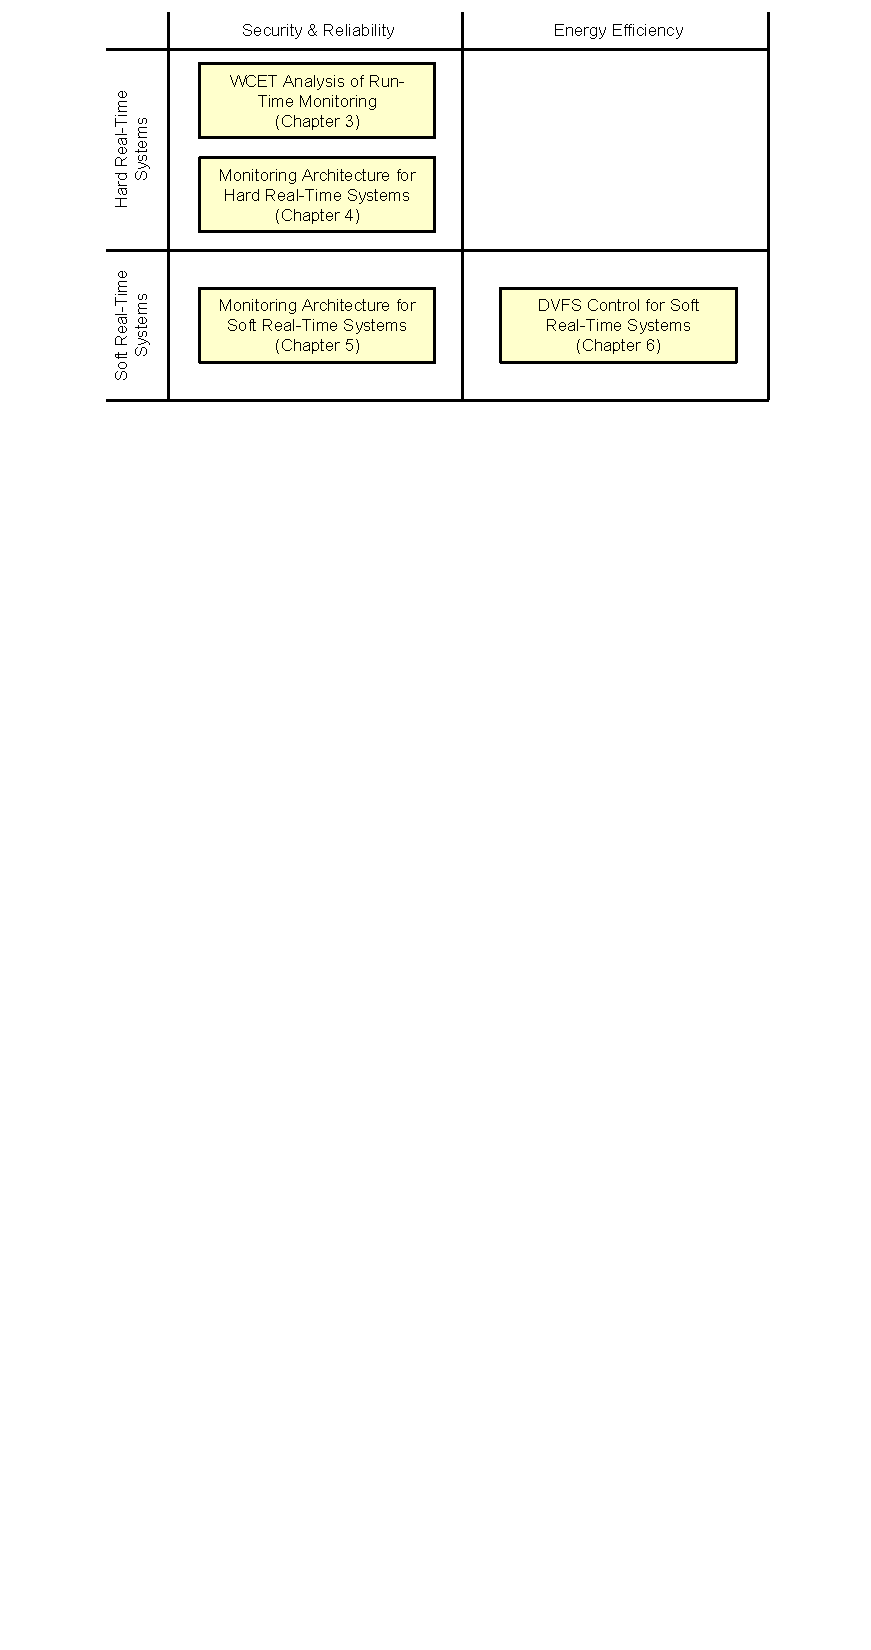
\includegraphics{figs/thesis_overview.pdf}
    \caption{Overview of techniques presented in this thesis.}
    \label{fig:intro.thesis_overview}
  \end{center}
\end{figure}


Figure~\ref{fig:intro.thesis_overview} shows an overview of the techniques
presented in this thesis.
The rest of the thesis is organized as follows.
Chapter~\ref{chap:background} discusses some background knowledge and
terminology that will be used throughout the thesis.
Chapters~\ref{chap:monitoring_wcet}, \ref{chap:monitoring_hard_drop}, and
\ref{chap:monitoring_dift_drop} discuss techniques on improving system security
and reliability through run-time monitoring on real-time systems. 
Chapter~\ref{chap:exec_time_prediction} presents predictive control of resource
allocation for creating energy-efficient real-time systems.
Finally, Chapter~\ref{chap:related_work}
discusses related work and Chapter~\ref{chap:conclusion} concludes the thesis.
